\documentclass{article}
\usepackage{graphicx}
\usepackage[utf8]{inputenc}
\usepackage[fleqn]{amsmath}
\usepackage{titling}
\usepackage{graphicx,wrapfig,lipsum}
\usepackage{amssymb}
\usepackage{listings}
\usepackage[font=small,labelsep=none]{caption}
\usepackage{array}% http://ctan.org/pkg/array
\usepackage{lipsum}
\usepackage{subcaption}
\usepackage{float}
\usepackage{hyperref}


\setlength{\droptitle}{-10em}

\title{Project 4}\vspace{-3ex}
\author{Benedicte Allum Pedersen, Emil Helland Broll and Fredrik Oftedal Forr}
\date{\vspace{-5ex}}

\begin{document}

\begin{titlepage}
  \centering
  
\includegraphics[width=0.15\textwidth]{./pics/uio.png}\par\vspace{1cm}
  {\scshape\LARGE Universitetet i Oslo\par}
  \vspace{1cm}
  {\scshape\Large Project 5\par}
  \vspace{1.5cm}
  {\huge\bfseries Making a model for the solar system using ordinary differential equations\par}
  \vspace{2cm}
  {\Large\itshape Benedicte Allum Pedersen, Fredrik Oftedal Forr og Emil Helland Broll\par}
	\vfill

  \vfill
  {\large 24. november 2019\par}
\end{titlepage}

\section*{Abstract}
We have used the velocity Verlet algorithm for solving coupled ordinary differential equations and object orientation for making a model for the soslar system. The equations we have used for this is based on Newton's law of motion due to the gravitational force. We found that the initial velocity at when the Earth start to escape the sun is 2.99$\pi$. 

\tableofcontents

\newpage

\section{Introduction}


\section{Method}

For a hypothetical solar system with only the Earth and the Sun Newton's law is given by one force $F_G$

\begin{flalign}
    F_G =\frac{GM_{\odot}M_E}{r^2}
    \label{eq:FG}
\end{flalign}

In the above equation $M_{\odot}$ and $M_E$ is the mass of the Sun and the Earth. G is the gravitational constant and r is the distance between the Earth and the Sun. We neglect the motion of the Sun and only look at the motion of the Earth relative to the Sun. We can do this because we assume that the mass of the Sun is much larger than the mass of the Earth. The gravitiational force consits of a x and y component $F_{G,x}$ and $F_{Gy}$, we then use Newton's second law and obtain:

\begin{flalign}
    \frac{d^2x}{dt^2} = \frac{F_{G,x}}{M_E} \ \
    \text{and} \ \
    \frac{d^2y}{dt^2} = \frac{F_{G,y}}{M_E}
    \label{eq:diff}
\end{flalign}

We use that the average distance bewteen the Earth and the Sun is $1.5 \cdot 10^{11}$ m and we call this one astronomical unit (1 AU). We use the masses of the different planets including the Sun that are given in \href{http://compphysics.github.io/ComputationalPhysics/doc/Projects/2019/Project5/SolarSystem/pdf/SolarSystem.pdf}{the description of Project 5}.

We introduce $x=r\ \cos(\theta), y = r\ \sin(\theta)$ and $r=\sqrt(x^2 + y^2)$. We can then rewrite

\begin{flalign*}
    F_x = - \frac{GM_{\odot}M_E}{r^2}cos(\theta) =  - \frac{GM_{\odot}M_E}{r^3} x \\
\end{flalign*}

and

\begin{flalign*}
    F_y = - \frac{GM_{\odot}M_E}{r^2}sin(\theta) =  - \frac{GM_{\odot}M_E}{r^3} y
\end{flalign*}

for the x and y direction of the gravitaional force. These to equations can again be rewritten so we obtain four first-order coupled differential equations

\begin{flalign*}
    \frac{dv_x}{dt} &= -\frac{GM_{\odot}}{r^3}x\\
    \frac{dx}{dt} &= v_x \\
    \frac{dv_y}{dt} &= - \frac{GM_{\odot}}{r^3}y\\
    \frac{dy}{dt} &= v_y
\end{flalign*}

By introducing astronomical units, described above(r = 1AU) and with the equation for circular motion, with $a = v^2/r$ we can set F=ma equal to the expression for the gravitaional force.

\begin{flalign*}
    \frac{M_Ev^2}{r} = F = \frac{GM_{\odot}M_E}{r^2}
\end{flalign*}

We then solve for $v^2r$, where $v$ is the velocity of Earth and when we assume circular motion we have $v=2\pir/yr = 2\piAU/yr$

\begin{flalign}
    v^2r = G M_{\odot} = 4\pi^2 \ \ AU^3/(yr)^2
    \label{eq:v2r}
\end{flalign}

where yr is short for years, which we use instead of seconds to decribe the motions in the solar system.

We can discretize the four coupled differential equations by using Euler's method with step length $h$.

\begin{flalign*}
    v_{x,i+1} &= v_{x,i} - h \frac{4\pi^2}{r_i^3}x_i , \\
    x_{i+1} &= x_i + hv_{x,i}, \\
    v_{y,i+1} &= v_{y,i} - h\frac{4\pi^2}{r_i^3}y_i, \\
    y_{i+1} &= y_i + hv_{y,i}
\end{flalign*}

\subsection{The Verlet-velocity method}
The Verlet method is a different numerical algorithm, where we again consider the second-order differential equation like Newton's second law, in one dimension this reads

\begin{flalign*}
    m \frac{d^2x}{dt} = F(x,t)
\end{flalign*}

which can be rewritten in terms of two coupled differential equations

\begin{flalign*}
    \frac{dx}{dt} = v(x,t) \quad and \quad \frac{dv}{dt} = F(x,t)/m = a(x,t)
\end{flalign*}

We perform a Taylor expansion of the discretized equations with step length $h$

\begin{flalign*}
    x(t+h) = x(t) + hx^{(1)}(t) + \frac{h^2}2x^{(2)}(t) + O(h^3)
\end{flalign*}

We know the second derivative from Newton's second law where $x^{(2)}(t) = a(x,t)$. By adding the Taylor expansion for $x(t-h)$ and by using the discretized expressions $x(t_i \pm h)= x_{i\pm1}$ and $x_i = x(t_i)$ we gets

\begin{flalign*}
    x_{i+1} = 2x_i - x_{i-1} + h^2x_i^{(2)} + O(h^4)
\end{flalign*}

where the truncation error goes like $O(h^4)$. We can also compute the velocity which has a truncation error $O(h^2)$

\begin{flalign}
    x_i^{(2)} = \frac{x_{i+1}-x_{i-1}}{2h} + O(h^2)
\end{flalign}

The Taylor expansion for the velocity is given by

\begin{flalign*}
    v_{i+1} = v_i + hv_i^{(1)} + \frac{h^2}{2}v_i^{(2)} + O(h^3)
\end{flalign*}

With Newton's second law we have

\begin{flalign*}
    v_i^{(1)}  = \frac{d^2x_i}{dt_i^2} = \frac{F(x_i,t_i)}m
\end{flalign*}

We add this to the derivative of the velocity

\begin{flalign*}
    v_{i+1}^{(1)} = v_^{(1)} + hv_i^{(2)} + O(h^2)
\end{flalign*}

Since our errors goes as $O(h^3)$ we obtain $hv_i^{(2)} \approx v_{i+1}^{(1)} - v_^{(1)}$. We rewrite the final equations for the position and the velocity and obtain

\begin{flalign*}
    x_{i+1} = x_i + hv_i + \frac{h^2}{2}v_i^{(2)} + O(h^3)
\end{flalign*}

and

\begin{flalign*}
    v_{i+1} = v_i + \frac{h}{2}\left(v_{i+1}^{(1)} v_i^{(1)} \right) + O(h^3)
\end{flalign*}

\subsection{Adding more planets to the binary system}

For a system with more than one planet we need to add the magnitude of the force between Earth and the other planet, for example jupiter which is the most massive planet in the solar system. This force is given by

\begin{flalign*}
    F_{Eart-Jupiter} = \frac{GM_{Jupiter}M_E}{r^2_{Earth-Jupiter}}
\end{flalign*}

where $M_{Jupiter}$ is the mass of Jupiter and $r_{Earth-Jupiter}$ is the distance between Earth and Jupiter. To extend the model for all the planets in the solar system we add the other planets in the same way and choose the initial positions and velocities for all the planets from \href{https://ssd.jpl.nasa.gov/horizons.cgi#top}{NASA}.


\subsection{Perihelion of Mercury}
The perihelion of a planet is the point where the planet in orbit around the Sun is closest to the Sun. The general theory of relativity explains the anomalous perihelion precession of the planet Mercury. The observed value for the perihelion precession when the classical effects are subtracted is 43''(43 arc seconds) per century. The behavior of the orbit around the sun will not be the same for each round, this means that the perihelion will slowly precess around the Sun and we would need to add a general relativistic correction to the Newton gravitaional force. The force then becomes:

\begin{flalign}
    F_G = \frac{GM_{Sun}M_{Mercury}}{r^2}\left[1 + \frac{3l^2}{r^2c^2} \right]
\end{flalign}

where $M_{Mercury}$ is the mass of Mercury and r is the distance bewteen the Sun and Mercury. The magnitude of the angular momentum is given by $l=|\vec{r} X \vec{v}|$ and c is the speed of light in vacuum. We obtain the perihelion angle $\thetha_p$ from the positions when Mercury is at its closest to the Sun, i.e the perihelion positions, $x_p$ and $y_p$. $\theta_p$ is then given by

\begin{flalign}
    tan \theta_p = \frac{y_p}{x_p}
\end{flalign}


\subsection{Programming}
    For this project, we perform our calculations in a C++ program, and make plots of the resulting data in Python. In order to simplify and make the program flexible, extendable and structured, we implement object orientation. We have also adapted the program to be able to simulate velocities and positions of planets and the Sun in both two and three dimensions.\\

    Our program consists of two classes – "System" and "Planet". "System" represents any system of bodies in the universe, allowing us to simulate unique systems with different initial properties and laws of physics. Our system can be modified to change the force of gravity's dependence on the inverse power of the distance between objects, through the factor $\beta$. In addition, we can decide whether or not the system should have a contributing force factor from relativistic forces. Finally, the "System" class has a function for performing Velocity Verlet-simulations over a given time span in order to simulate the movement of the planets over time. We also have a function that looks at the perihelion precession and the perihelion angle of a system.\\
    "Planet" represents any object that can be added to the system. The bodies we look at are mainly the Sun and the Earth, but also Jupiter, Mercury and the rest of the planets, in different parts of this project. The "Planet" class initializes the planet with an initial position and velocity in space in astronomical units (AU and AU/day), and a mass relative to the Sun. The "Planet" class also includes several functions for calculating distances between objects in (our outside of) a system, and forces, acceleration and energy of the planet.\\

    This object oriented structure allows us to easily simulate different systems we are interested in. Looking at how the orbit of the Earth and Jupiter around the Sun changes when the mass of Jupiter changes can then be done in just a few lines of code, in a simulator program utilizing the "System" and "Planet" classes.\\

    In order to simulate a system with the sun in a constant position, we make sure that, for each step in the Velocity Verlet calculation, to calculate the velocities of the planets relative to the velocity of the Sun. This ensures that the Sun never has a velocity, so that we fix the movements of the planets relative to each other. In order to simplify, we chose to do this instead of manually adjusting for the center of mass of the system, as this would make the logic more complicated. This functionality is optional, and can be turned off easily in the creation of the "System" object.\\

    Finally, we have several Python programs for plotting the calculated data of the system, allowing for both 2D and 3D plots, with black backgrounds and no ticks on the axes, as this would not be very relevant in the final report. We made different programs for plotting a single system and for plotting several systems in one plot. All the plotting programs assume the Sun's position is in origo, and unchanging, in order to be able to produce plots from large data sets, although we can easily modify the program to plot the Sun with a changing position, as the data files (optionally) can include the Sun's position as well.  


\section{Results}
We have solved equation \ref{eq:v2r} using both Euler's forward algorithm and the velocity Verlet method. We saw that Euler's algorithm requiers a lot more calculation steps to become accurate than the Verlet algorithm. Euler's algorithm requires $5 \cdot 10^6$ steps while the Verlet algorithm requires only 500 steps. If we run our code with 100 000 integration points Euler takes 23.8 ms and uses 17 N flops while Verlet uses 35.7 ms with 38 N flops. We have therefore used the velocity Verlet method to calculate and plot the position, the energy and the angular momentum of the Earth. The results can be found in Figure \ref{fig:position}, \ref{fig:energy} and \ref{fig:am}. The plot of the energy(Figure\ref{fig:energy}) is obtained by a sum of the potential and the kinetic energy. From these figures we can see that the energy and the angular momentum is conserved. These properties is consereved because if they were not conserved the Earth would not be in orbit with around the Sun.

\begin{figure}[H]
    \begin{center}
        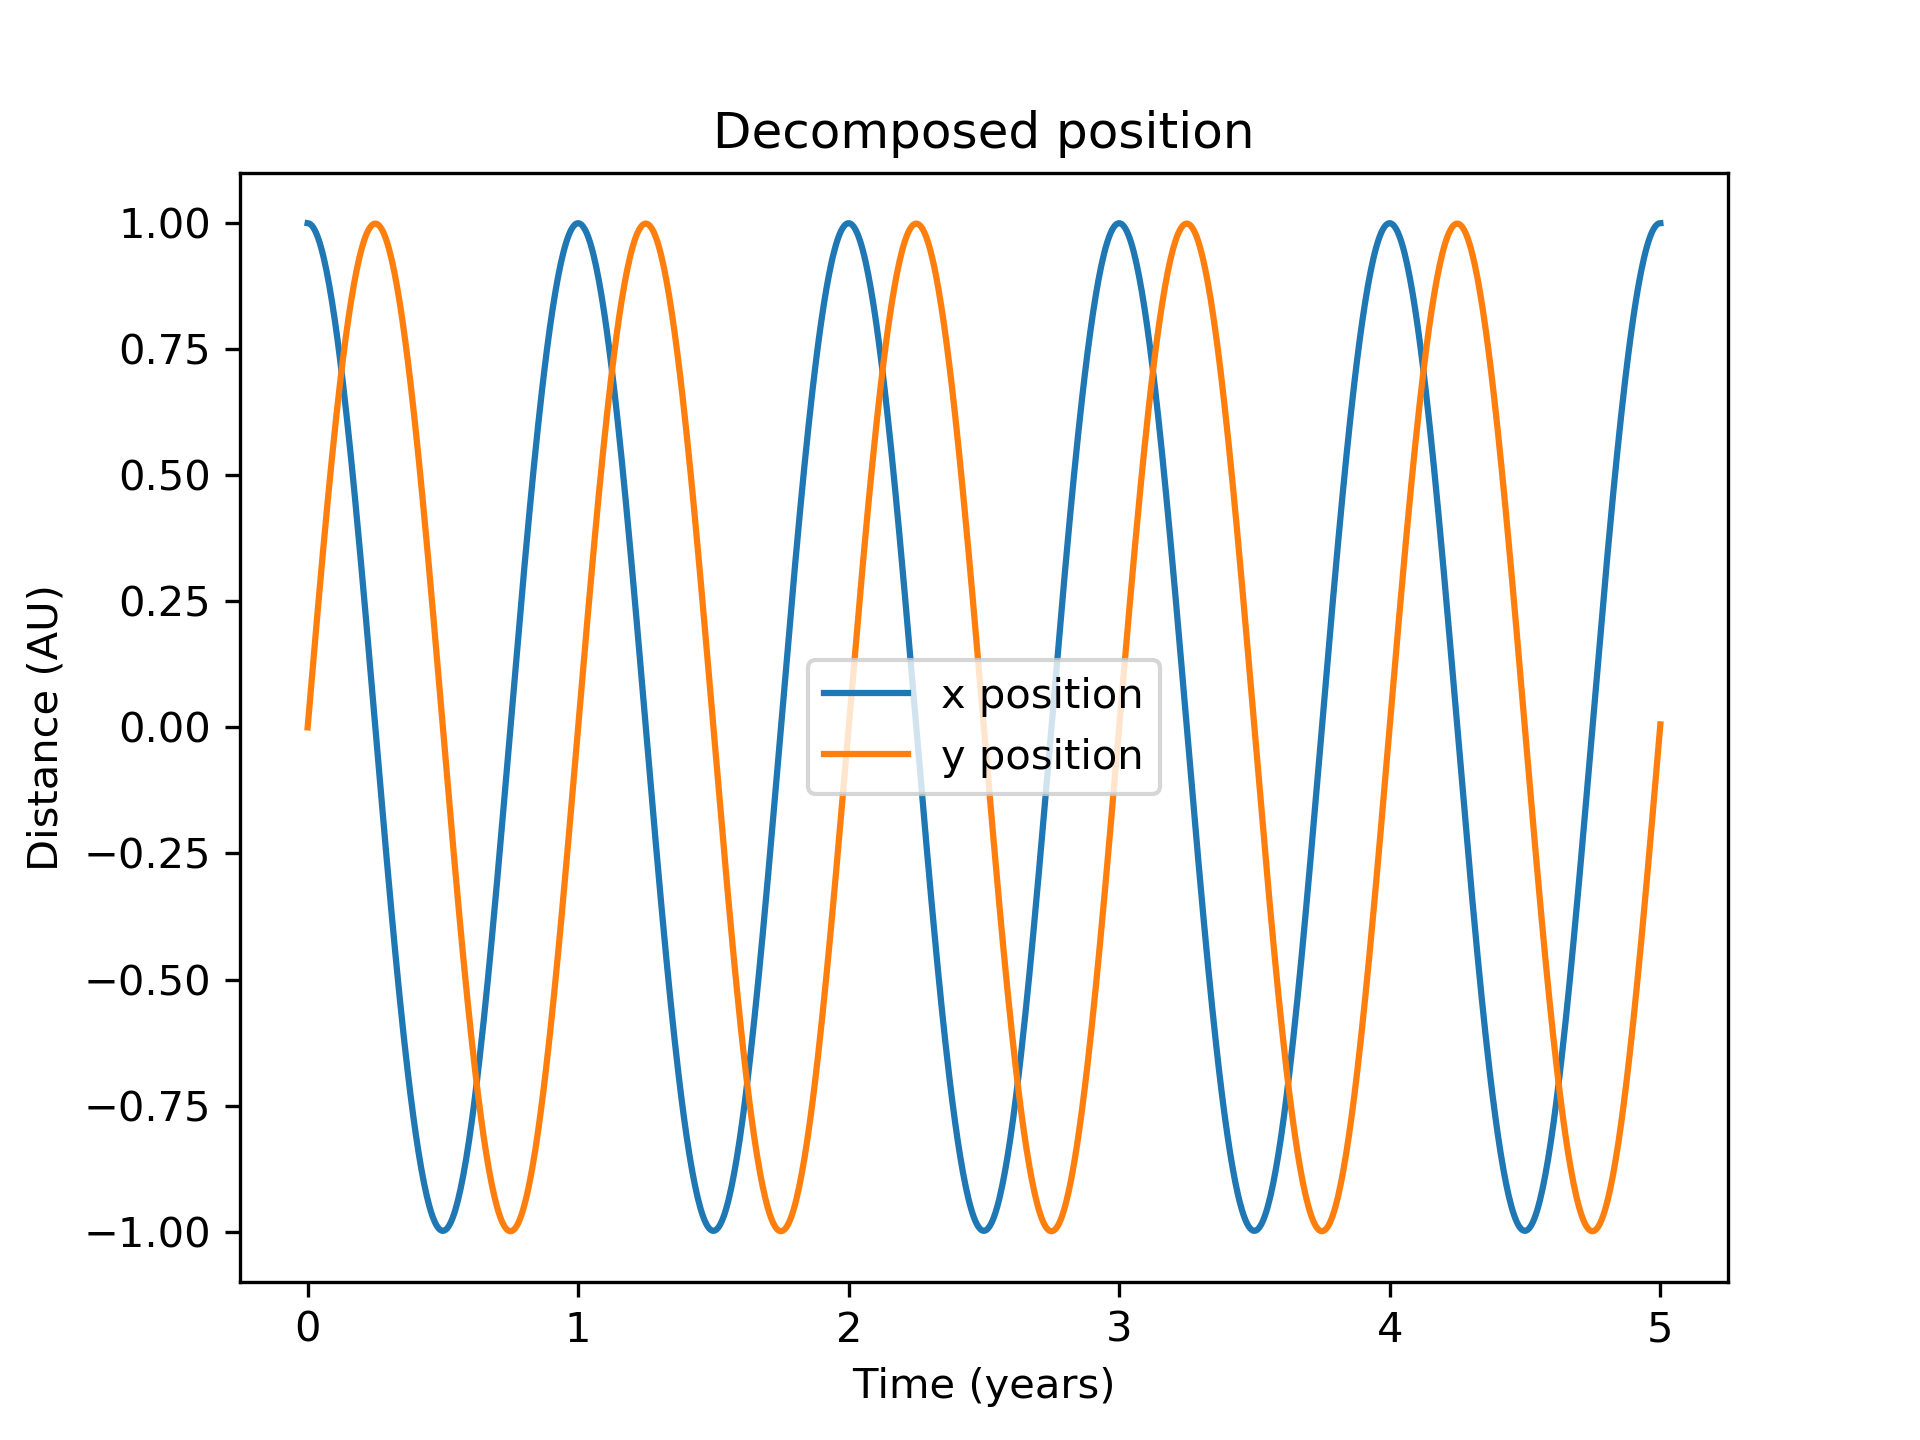
\includegraphics[width=0.8\textwidth]{./Plot/xy_vs_time.png}
        \caption{: }
        \label{fig:position}
    \end{center}
\end{figure}

\begin{figure}[H]
    \begin{center}
        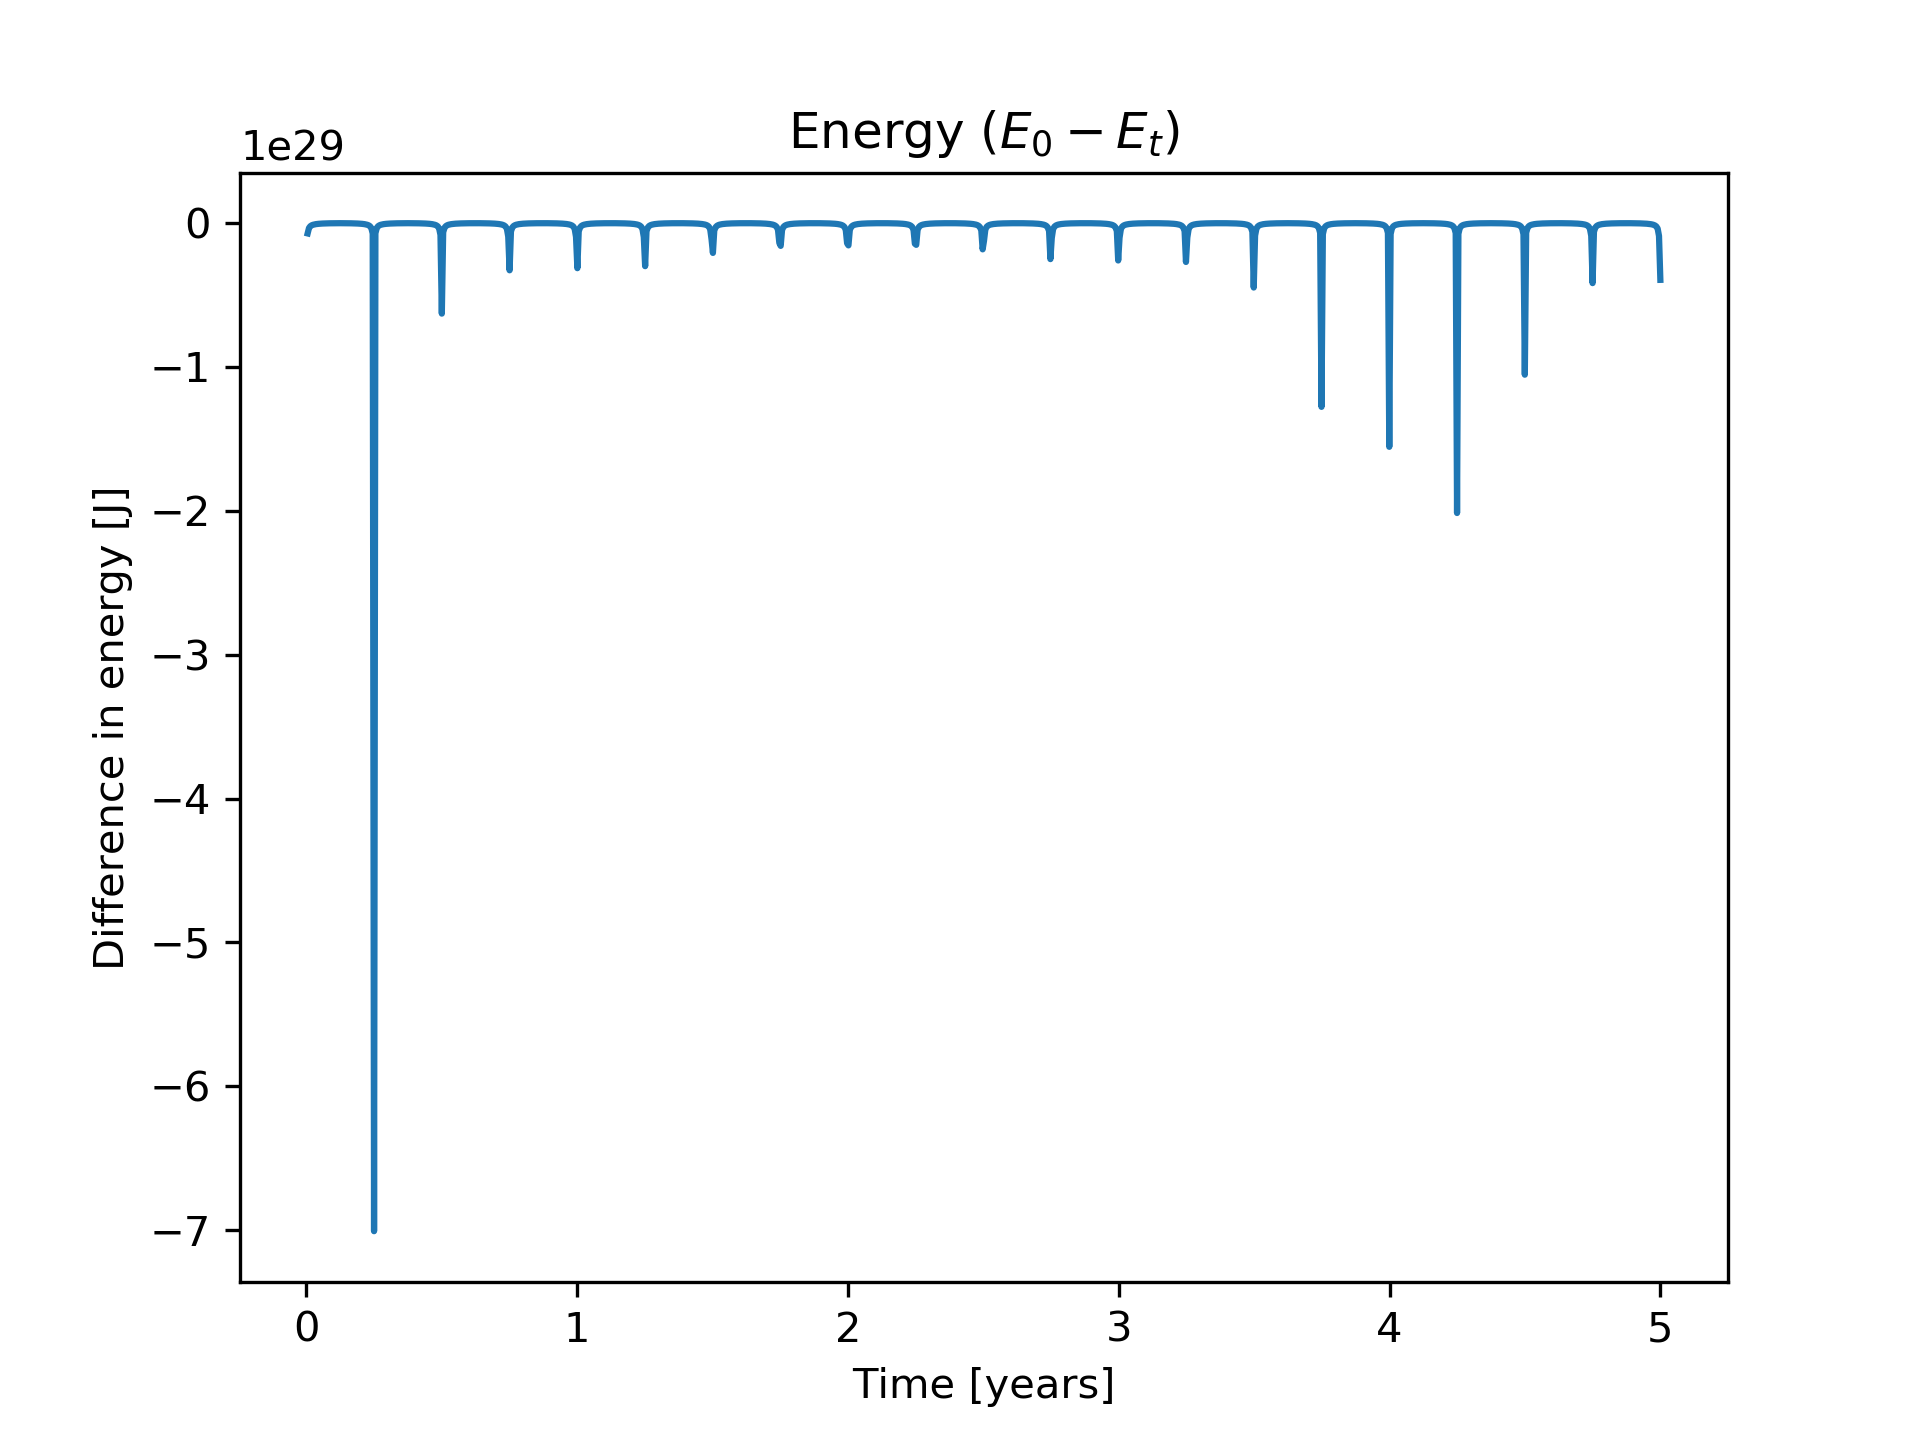
\includegraphics[width=0.8\textwidth]{./Plot/energy.png}
        \caption{: Energy}
        \label{fig:energy}
    \end{center}
\end{figure}

\begin{figure}[H]
    \begin{center}
        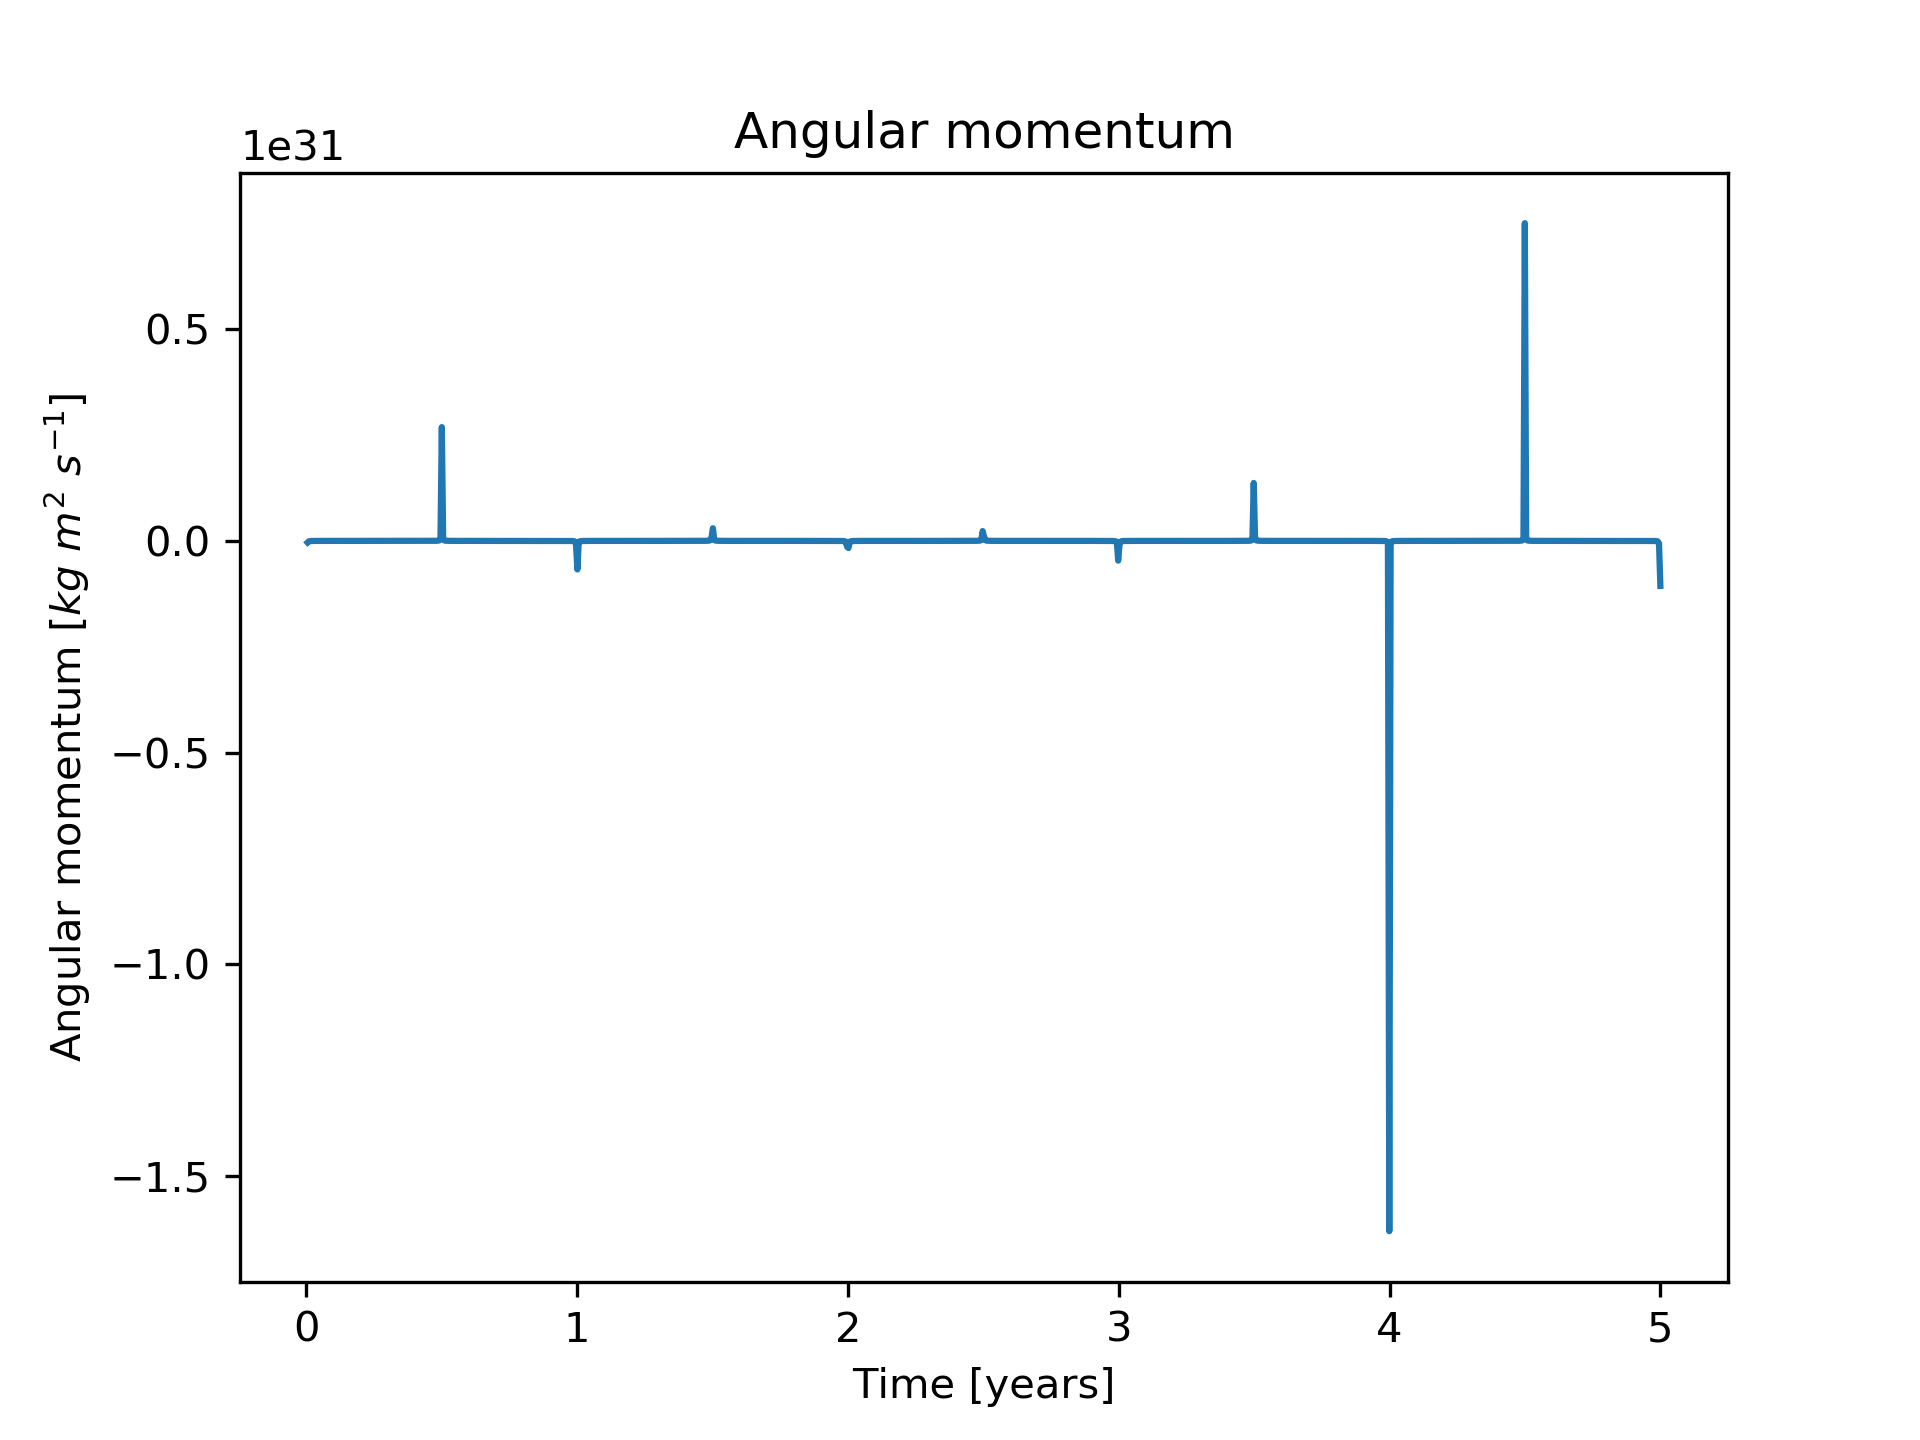
\includegraphics[width=0.8\textwidth]{./Plot/angular_momentum.png}
        \caption{: Angular Momentum}
        \label{fig:am}
    \end{center}
\end{figure}

\subsection{Initial velocity for circular orbit}
The initial velocity needs to be minimum 2$\pi$ AU/(yr) to obtain a circular orbit of the Earth around the Sun. We have seen this both in our code but we can also see this in the mathematics.

\begin{flalign*}
    \frac{mv^2}r &= \frac{GM_{\odot}M_E}{r^2}\\
    v^2 &= \frac{GM_{\odot}}r\\
    v &= \sqrt{\frac{4\pi^2}1} = 2\pi
\end{flalign*}

The plot of the Earth's orbit around the Sun is shown in Figure \ref{fig:earth_orbit}

\begin{figure}[H]
    \begin{center}
        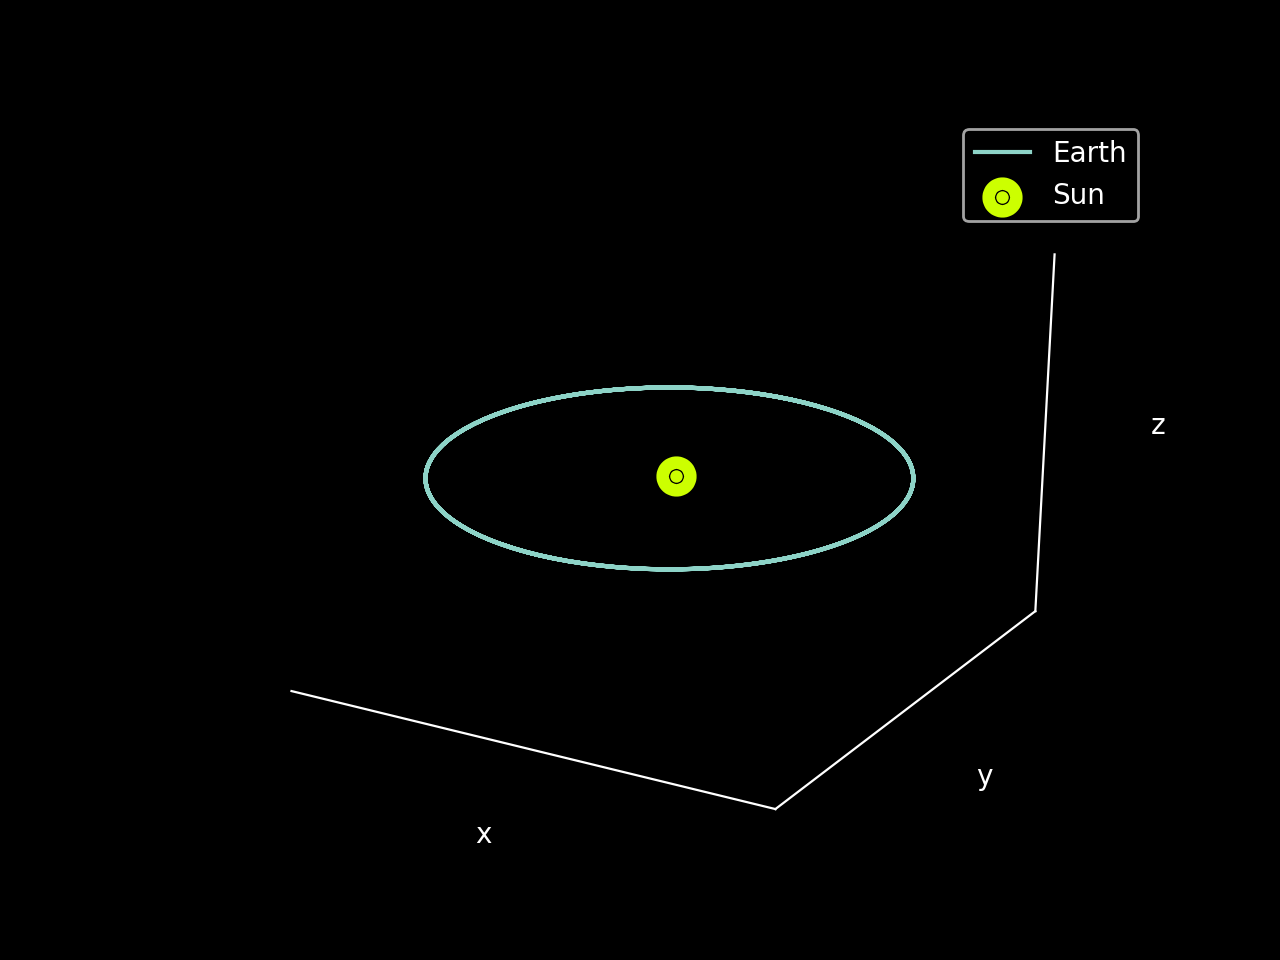
\includegraphics[width=0.8\textwidth]{./Plot/Earth_orbit.png}
        \caption{: Plot of the orbit of the Earth around the Sun.}
        \label{fig:earth_orbit}
    \end{center}
\end{figure}

\subsection{Escape velocity}
We then consider a planet which begins at a distance 1 AU from the Sun, the inital velocity at when the planets begin to escape from the Sun is at 2.79$\pi$ AU/(yr), this means that at this inital velocity the planets orbits is no longer circular. Figure \ref{fig:last} shows the last orbit with this stable initial velocity before the Earth escapes from the Sun.

\begin{figure}[H]
    \begin{center}
        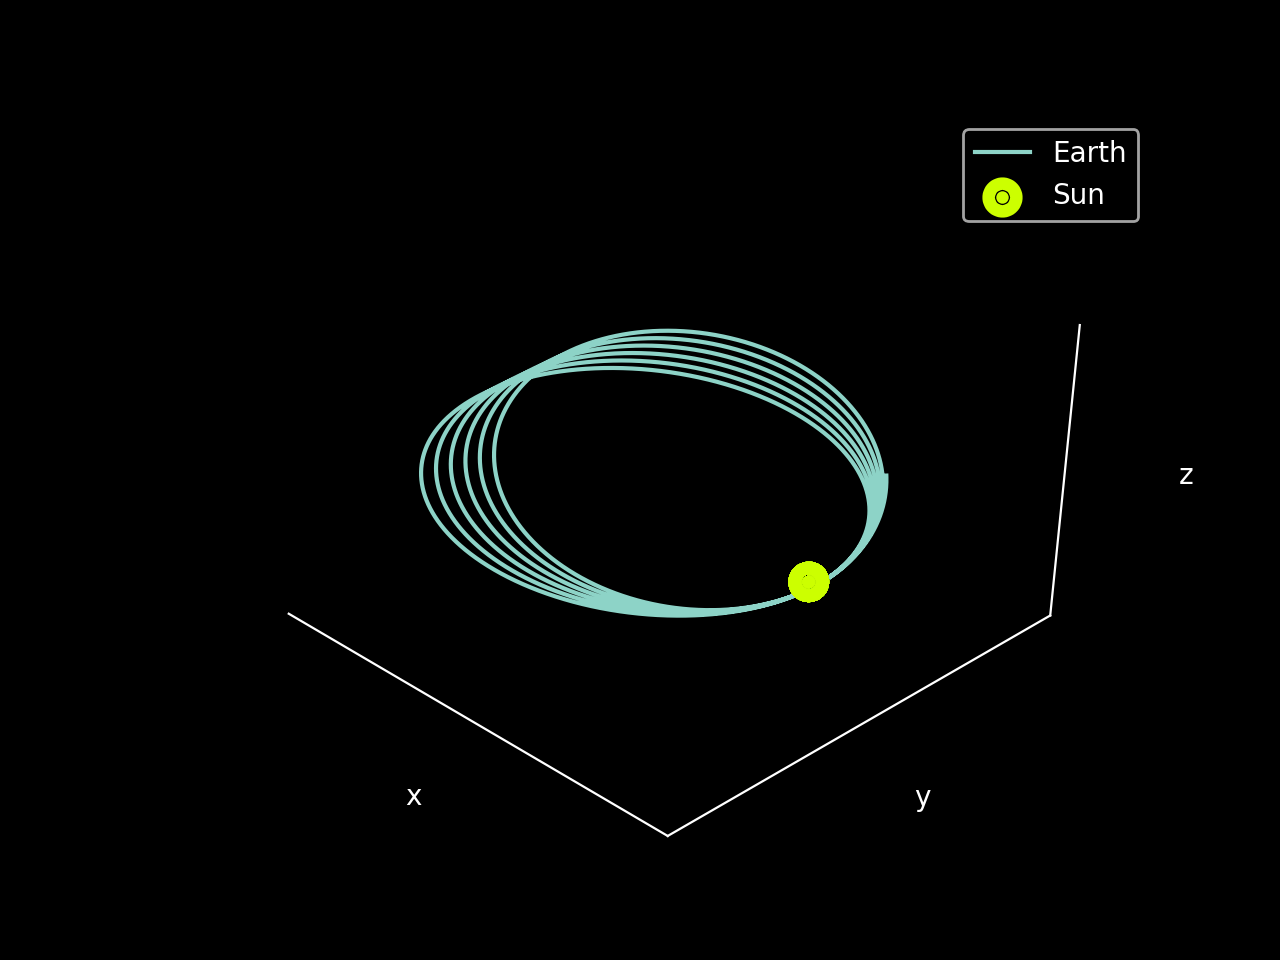
\includegraphics[width=0.8\textwidth]{./Plot/last_stable_orbit.png}
        \caption{: Plot of Earth's orbit around the sun before it escapes the sun.}
        \label{fig:last}
    \end{center}
\end{figure}

This numerical value is quite accurate compared to the exact value. We can calculate this escape velocity exact by considering the work needed to move a planet over a small distance dr against the attractive force the planet feels. This work is given by:

\begin{flalign*}
    dW &= F_G dr = -\frac{GM_{\odot}M_E}{r^2}\\
    W &= \int_r_0^\infty - G\frac{M_{\odot}M_E}{r^2} = -G \frac{M_{\odot}M_E}{r_0}
\end{flalign*}

This gives the minimal kinetic energy to be able to reach infinity, therefore the escape velocity $v_0$ satisfies

\begin{flalign*}
    W + K &= 0 \rightarrow \frac{1}2 M_Ev_0^2 = G\frac{M_{\odot}M_}{r_0}\\
    v_0 &= \sqrt{\frac{2GM_{\odot}}{r_0}} = \sqrt{2\cdot4\pi^2} AU/yr = 2.8\pi AU/yr
\end{flalign*}

\subsection{Changing the gravitaional force}
If we try to replace the gravitaional force from Equation \ref{eq:FG} with

\begin{flalign*}
    F_G = \frac{GM_{\odot}M_E}{r^{\beta}}
\end{flalign*}

with $\beta \in [2,3]$. The results is shown in Figure \ref{fig:beta}. These figures shows that when $\beta$ approches 3 the Earth begins to escape the sun. This would have been the case if the gravitaional force worked different, so we are lucky since the gravitaional force keeps us in orbit around the Sun.

\begin{figure}[H]
    \makebox[\textwidth]{\makebox[1.5\textwidth]{%
    \begin{subfigure}{.5\textwidth}
            \centering
            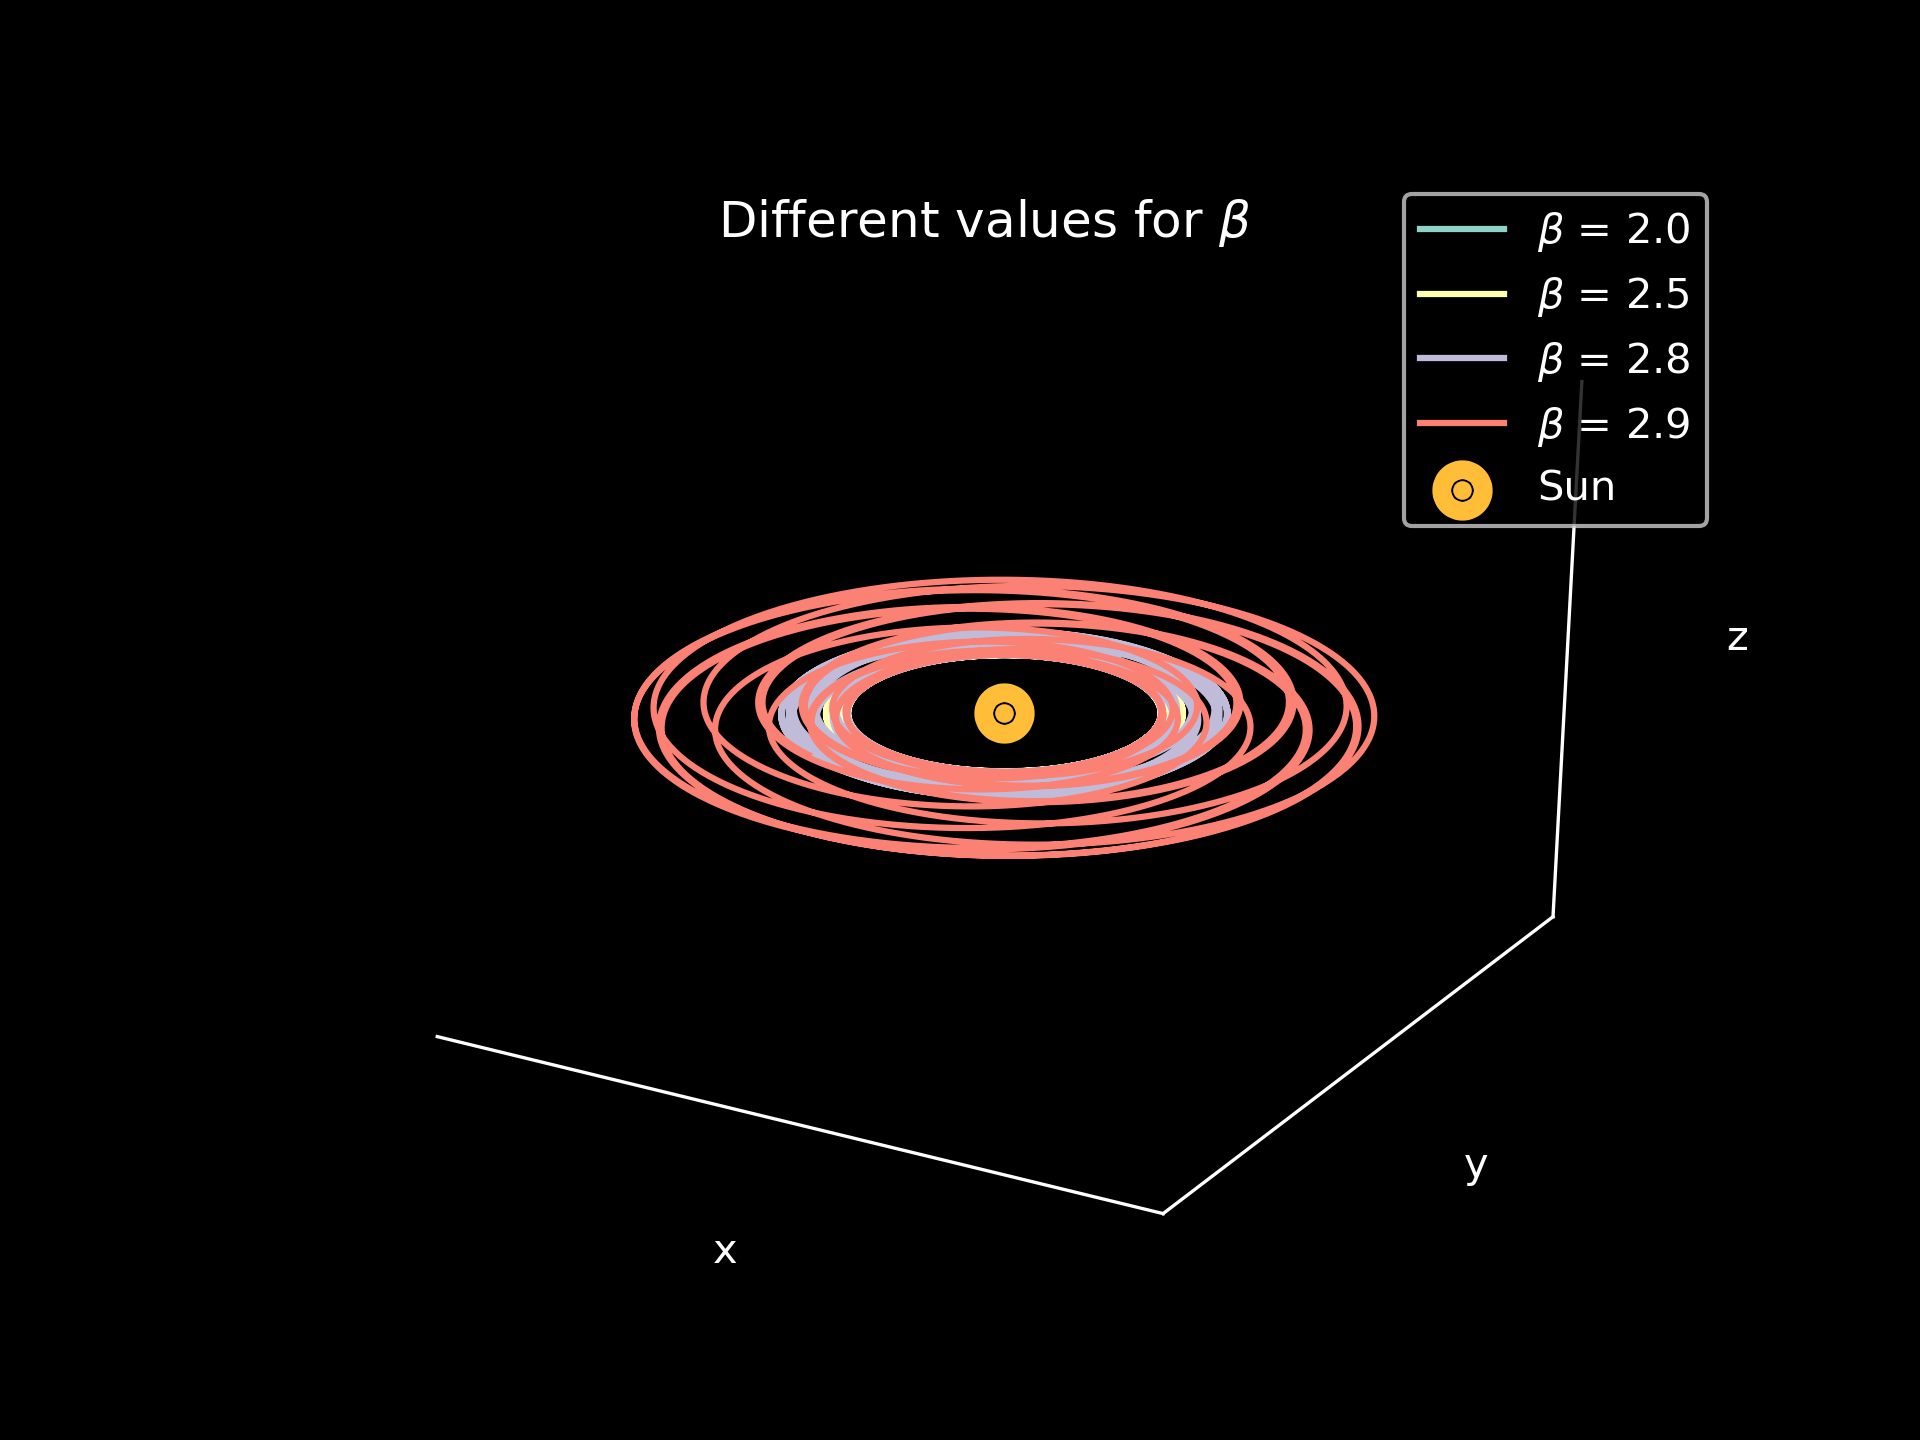
\includegraphics[width=250px]{./Plot/vary_beta_1.png}
            %\caption{}
    \end{subfigure} \hfill %
    \begin{subfigure}{.5\textwidth}
            \centering
            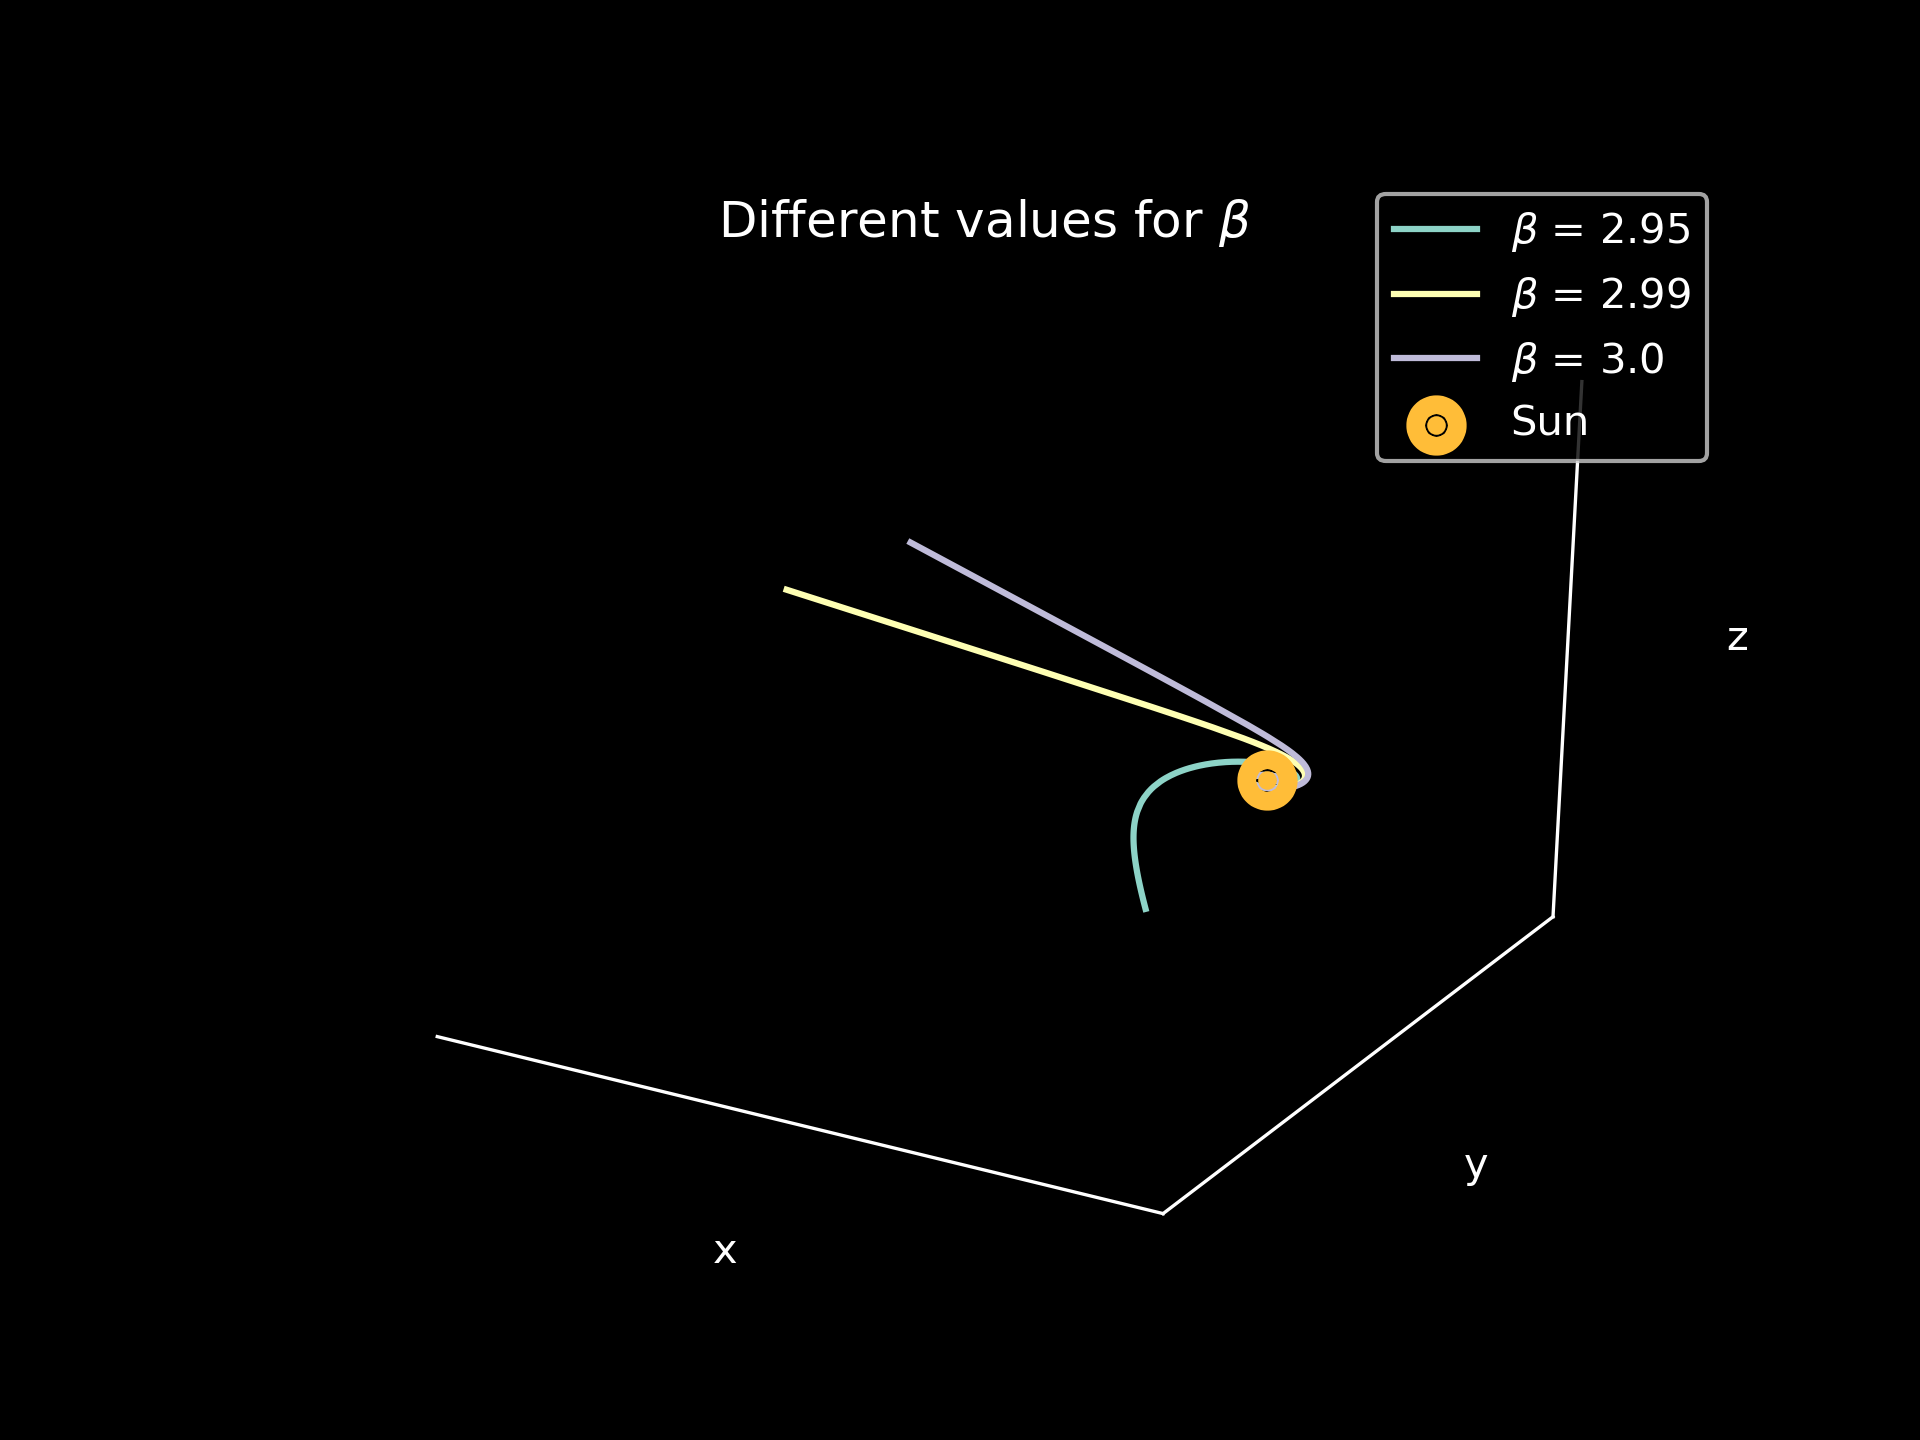
\includegraphics[width=250px]{./Plot/vary_beta_2.png}
            %\caption{}
    \end{subfigure}\hfill}}
    \caption{: The Earth-Sun system for different values of $\beta$.}
    \label{fig:beta}
    \end{figure}

\subsection{Adding Jupiter to the system}
We then add Jupiter to our system and we evaluate how it affects our system when we increase Jupiters mass. The result when Jupiter has it's own mass is shown in Figure \ref{fig:jupiter1}. When we increase the mass with a factor of 10 the result does not differ from what we see in Figure \ref{fig:jupiter1}. Figure \ref{fig:jupiter} shows what will happen when we increase the mass of Jupiter with a factor of respectively 950 and 1000. These figures shows that when the mass of Jupiter gets large it will attract the Earth away from its normal orbit around the Sun. When we increse the mass with a factor of 1000 the Earth will escape the sun because the repulsive force bewteen Jupiter and the Earth become really big. When Jupiter's mass is increased with a factor of 1000 we needed about 20 000 steps for the system to be stable, that is equivalent to approximately 20 years.

\begin{figure}[H]
    \begin{center}
        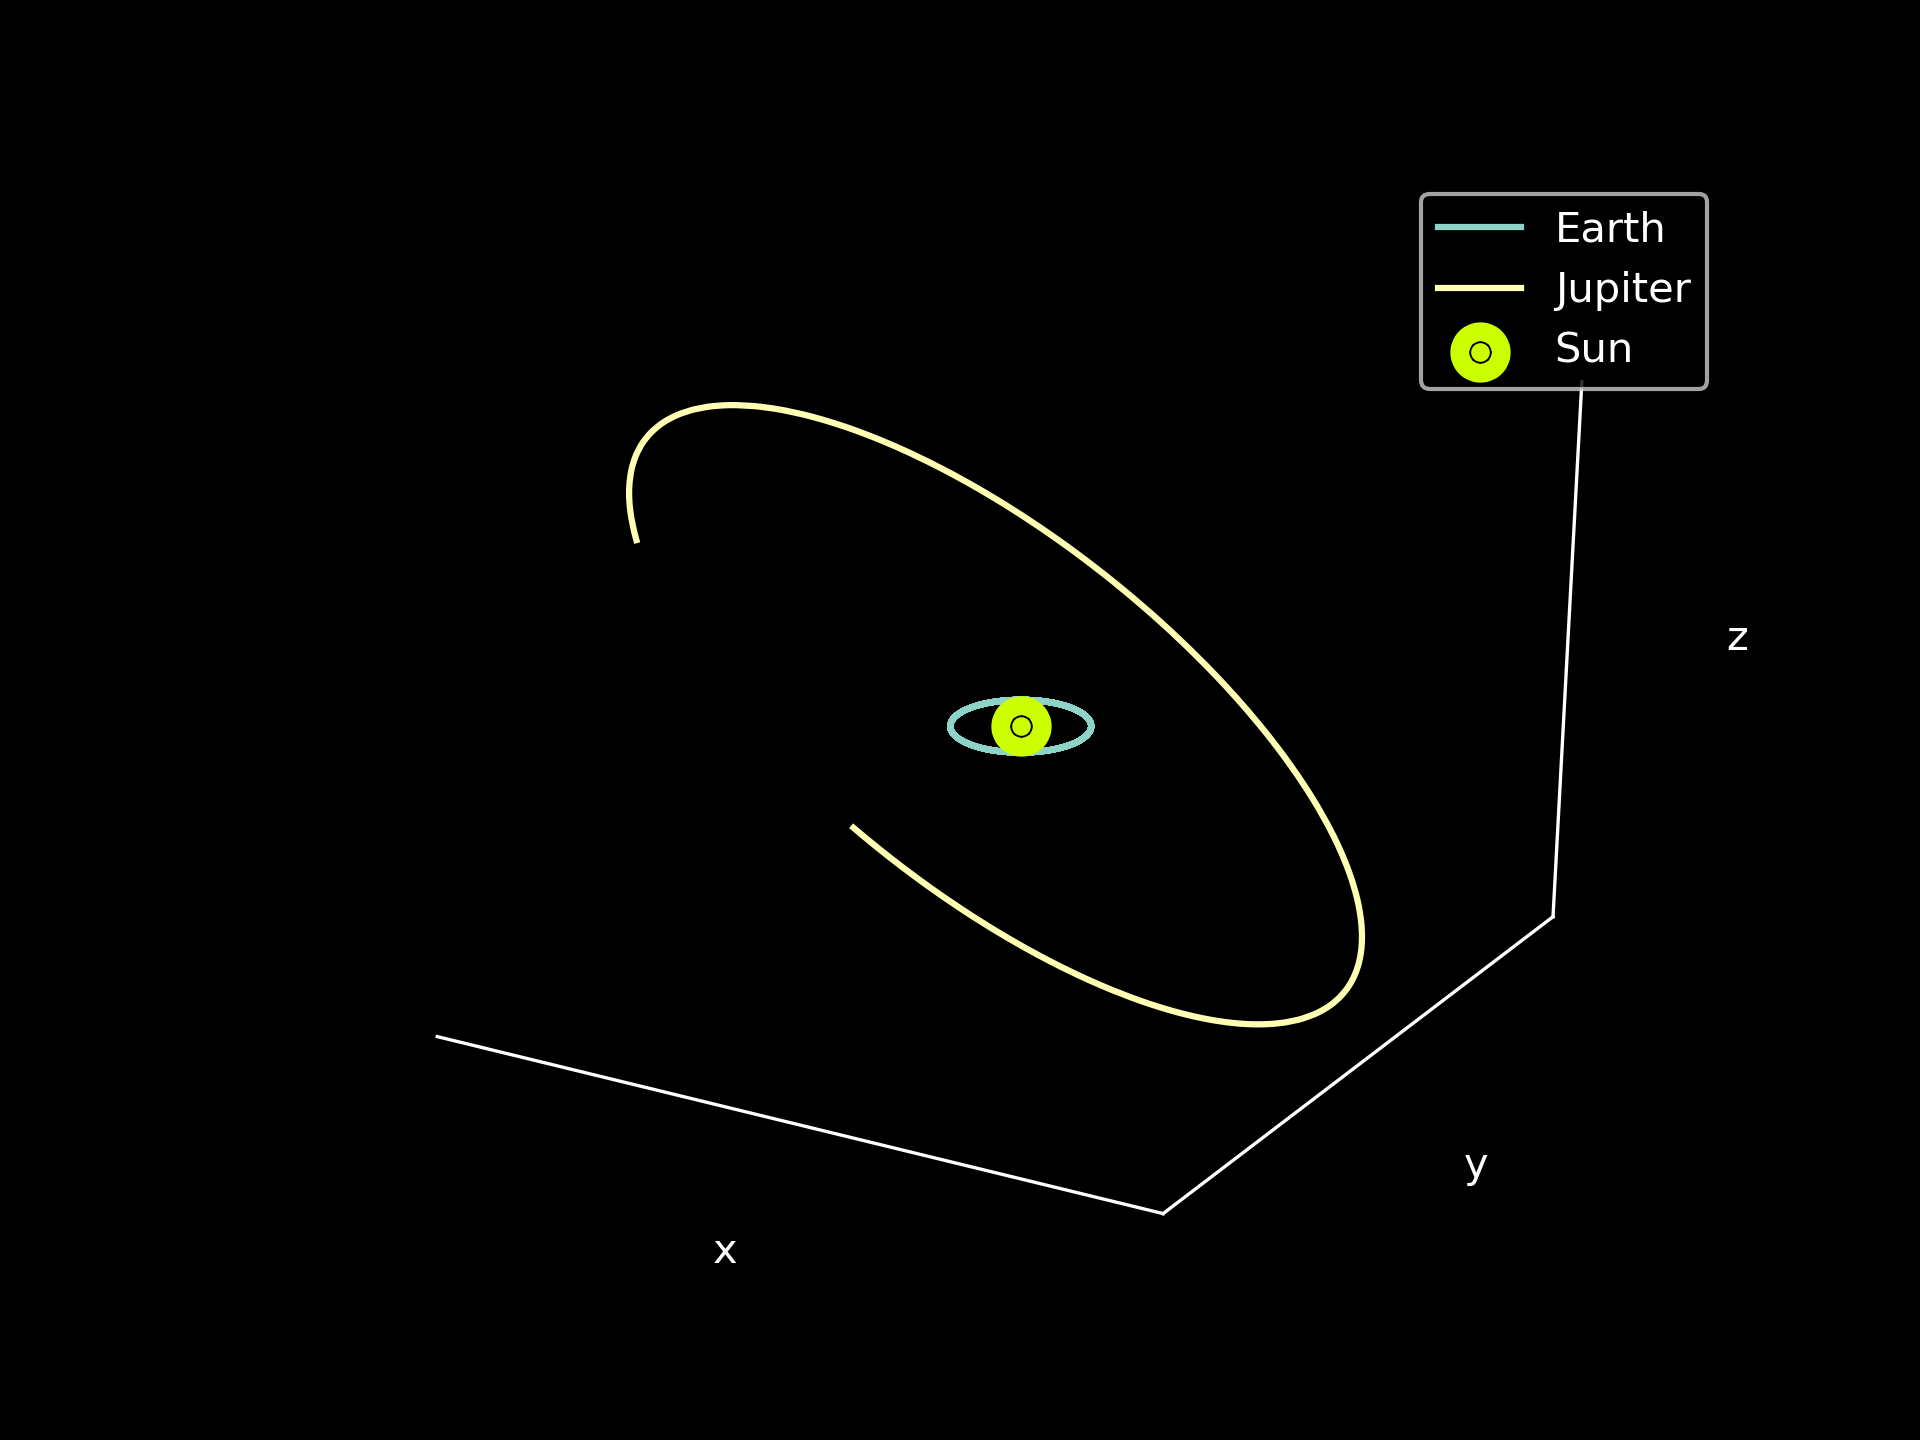
\includegraphics[width=0.8\textwidth]{./Plot/Earth_Jupiter1.png}
        \caption{: Solar system including Earth and Jupiter.}
        \label{fig:jupiter1}
    \end{center}
\end{figure}

\begin{figure}[H]
    \makebox[\textwidth]{\makebox[1.5\textwidth]{%
    \begin{subfigure}{.5\textwidth}
            \centering
            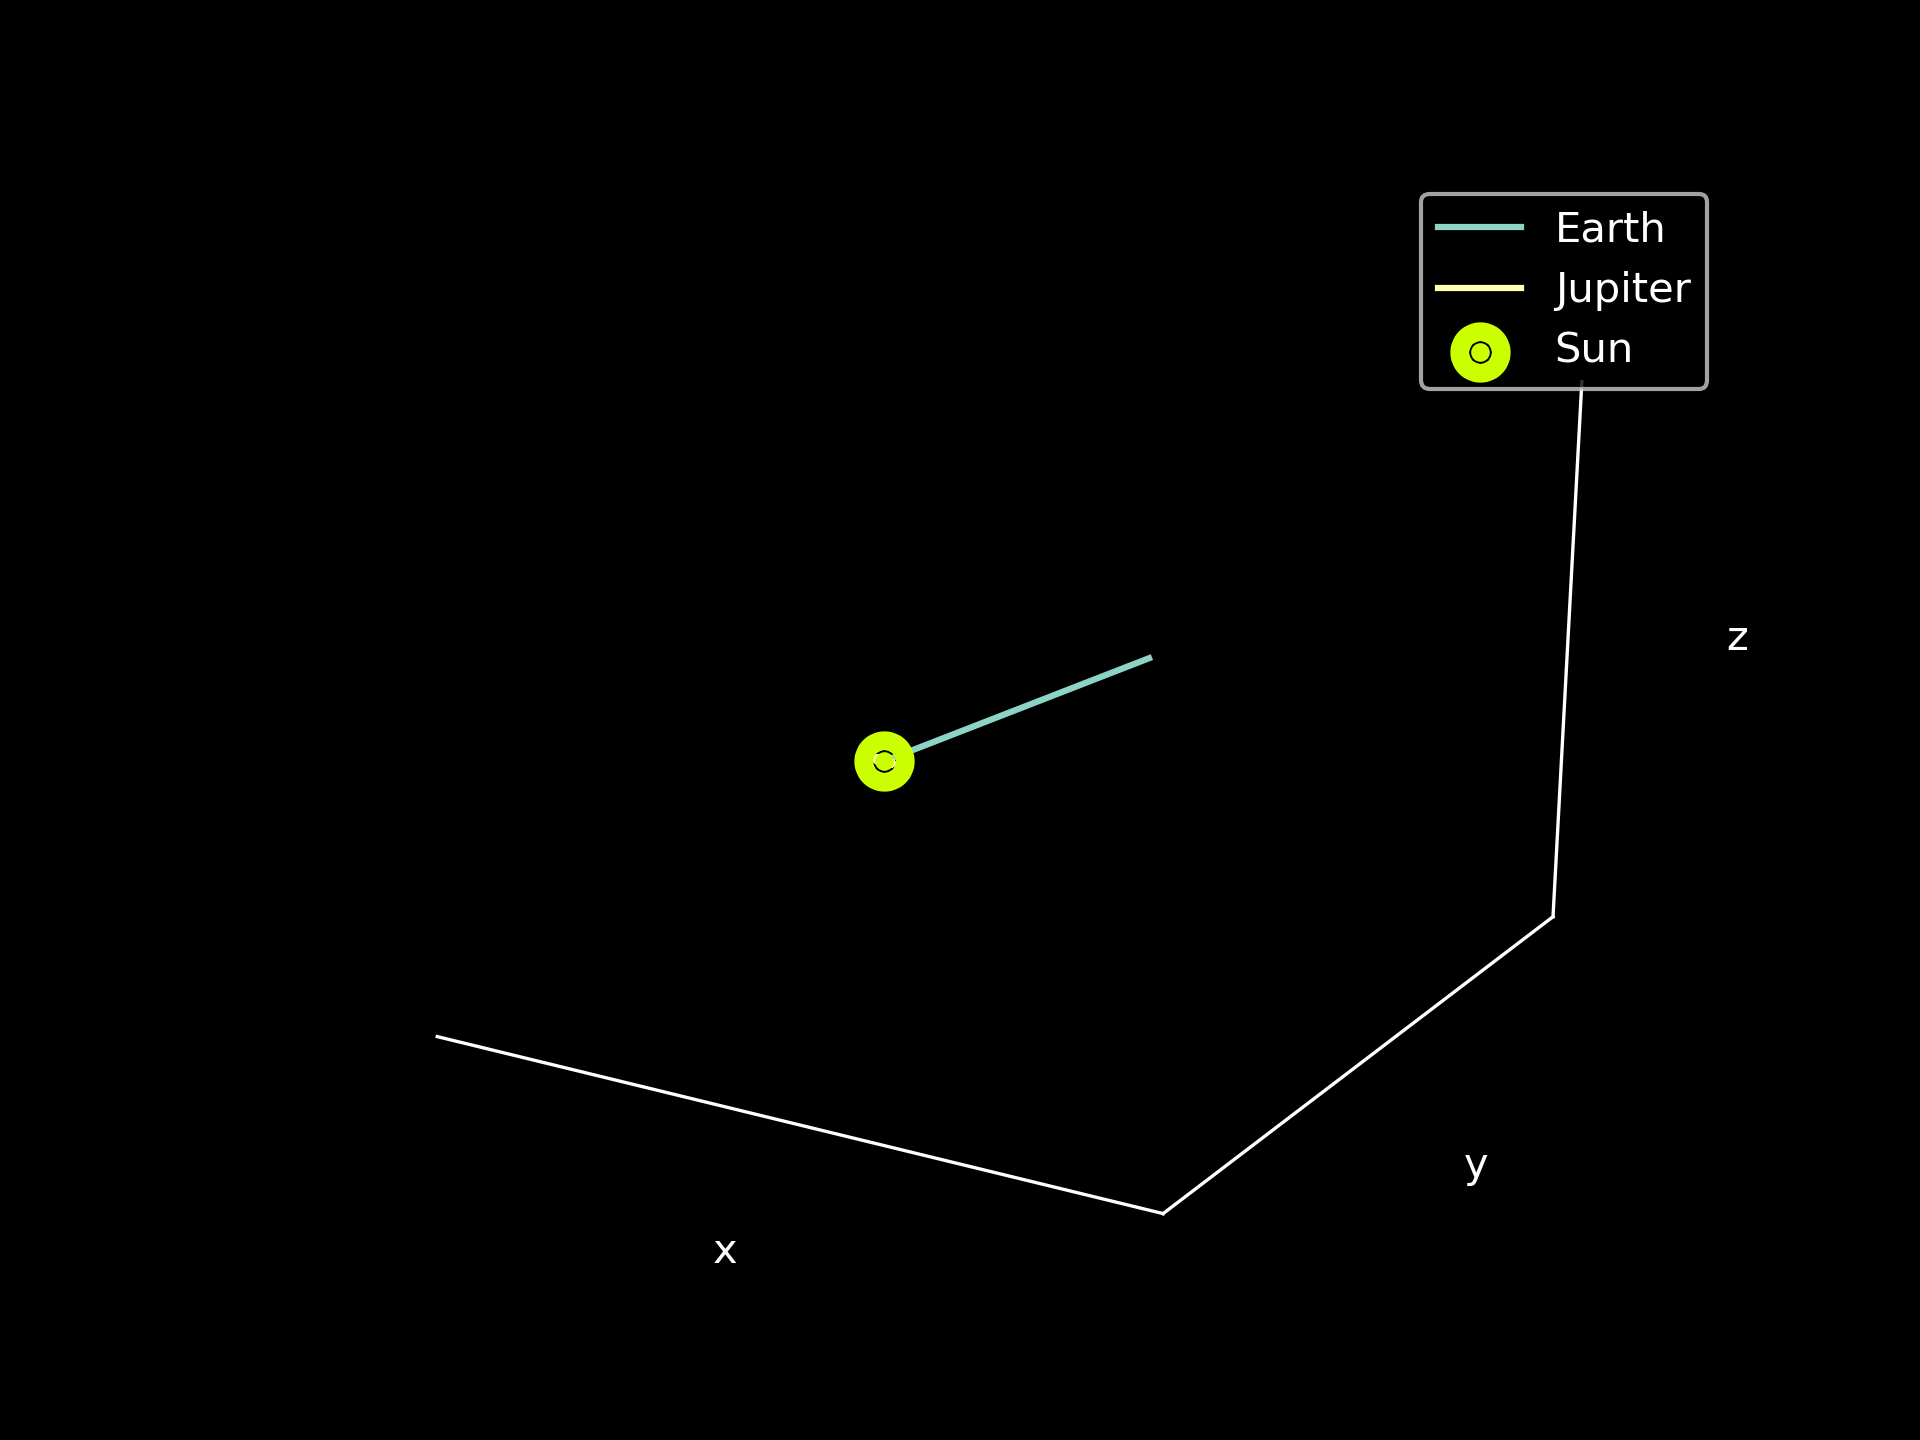
\includegraphics[width=250px]{./Plot/Earth_Jupiter950.png}
            \caption{Mass of Jupiter increased with a factor of 950}
    \end{subfigure} \hfill %
    \begin{subfigure}{.5\textwidth}
            \centering
            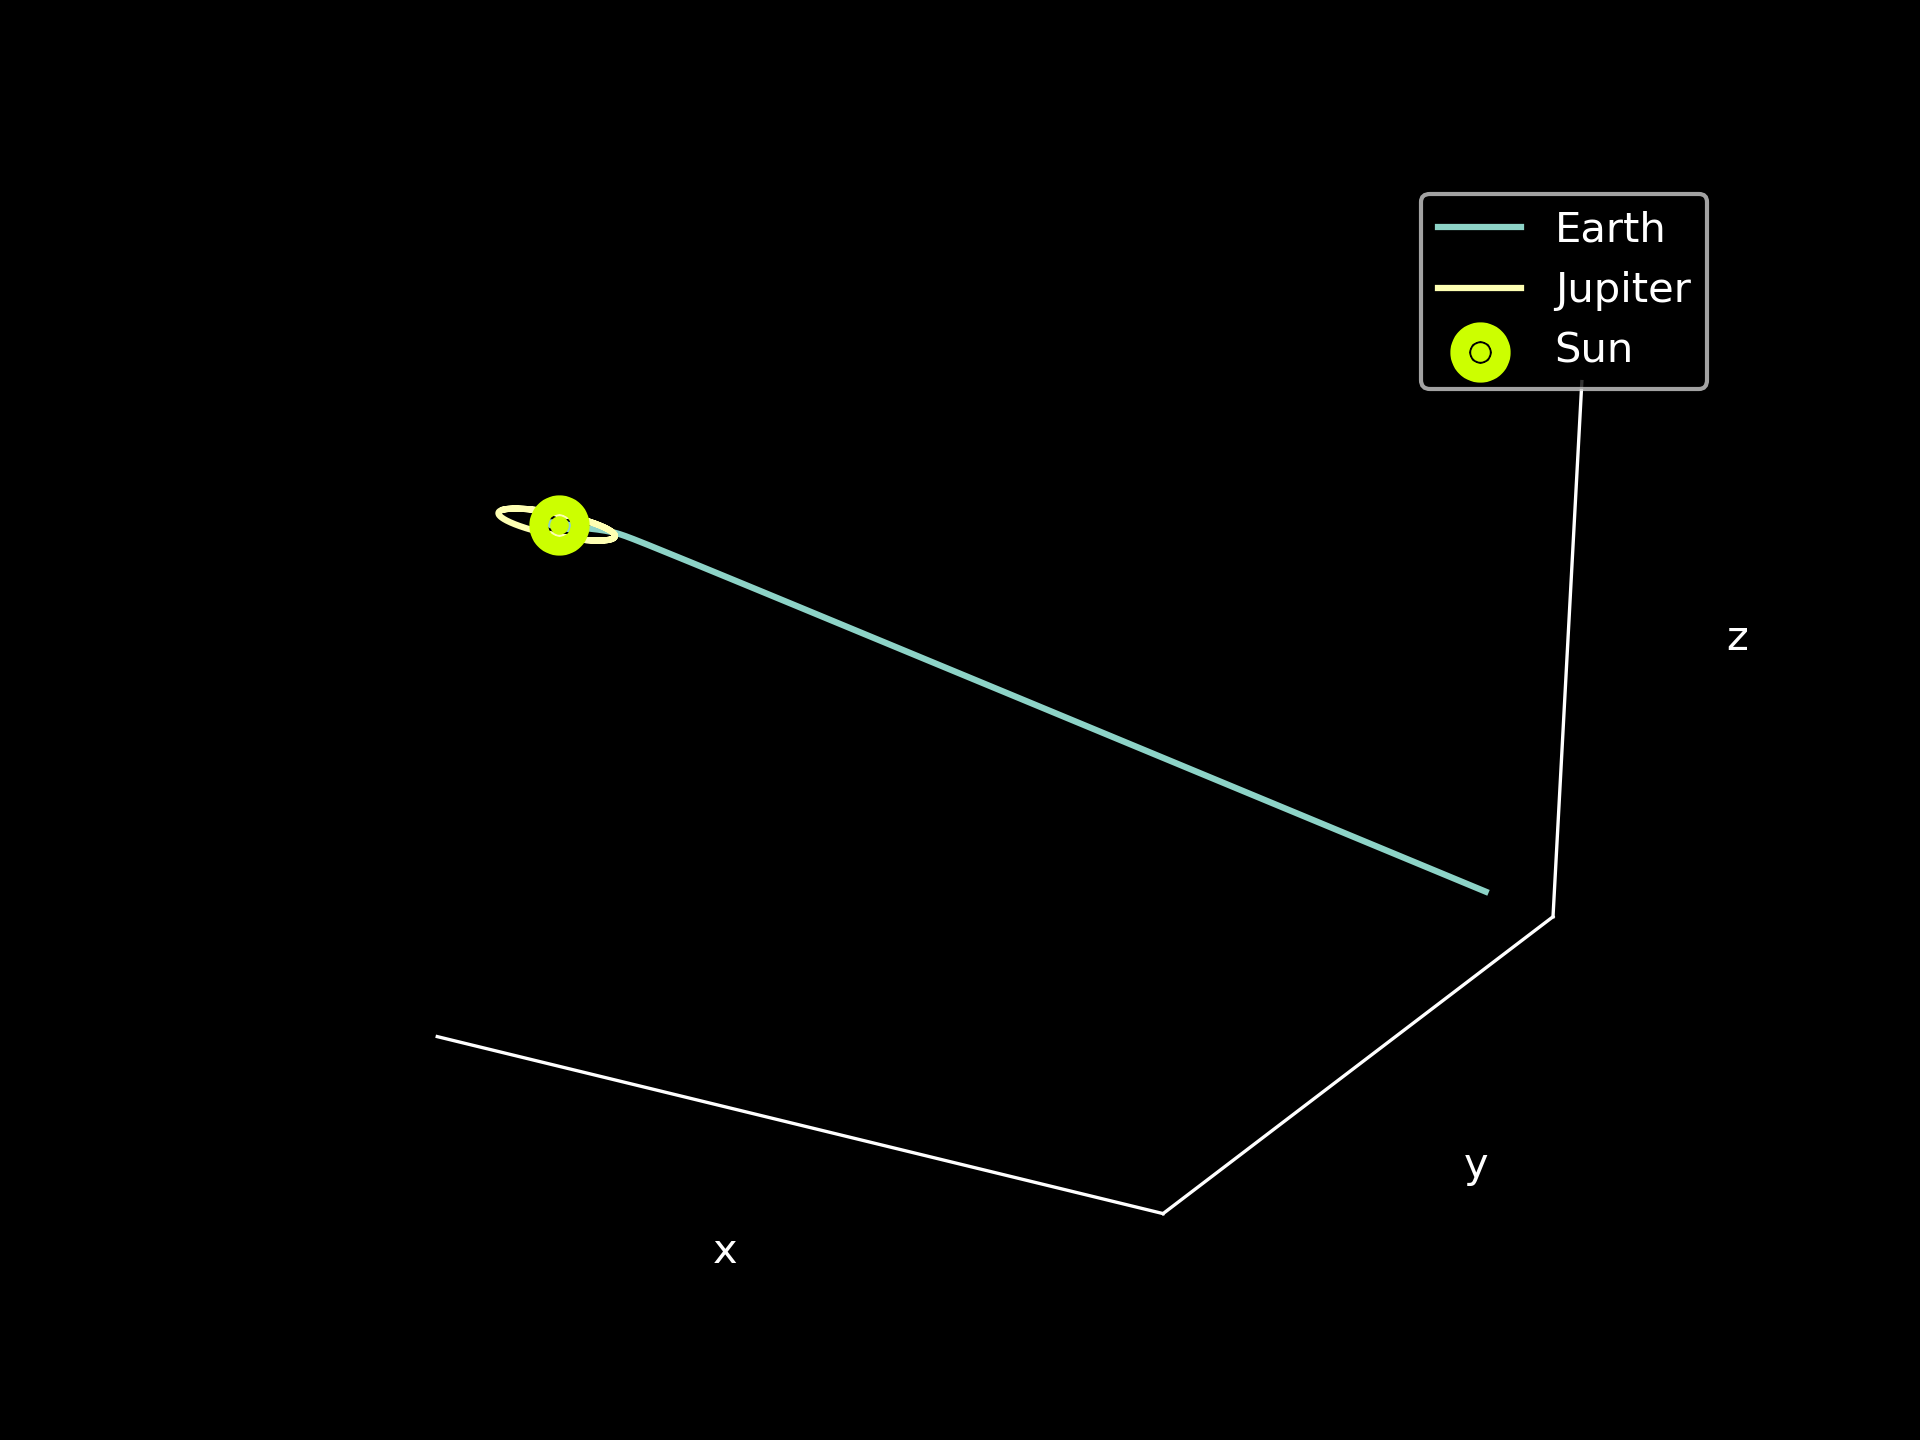
\includegraphics[width=250px]{./Plot/Earth_Jupiter1000.png}
            \caption{Mass off Jupiter increased with a factor of 1000}
    \end{subfigure}\hfill}}
    \caption{: Solar system including Earth and Jupiter, with the mass of Jupiter increased.}
    \label{fig:jupiter}
    \end{figure}

\subsection{Finished solar system}
Further we have completed the whole solar system by adding more planets, we have plottet this with 500 000 integration points and over 164 years. The results is represented in Figure \ref{fig:solar}.

\begin{figure}[H]
    \begin{center}
        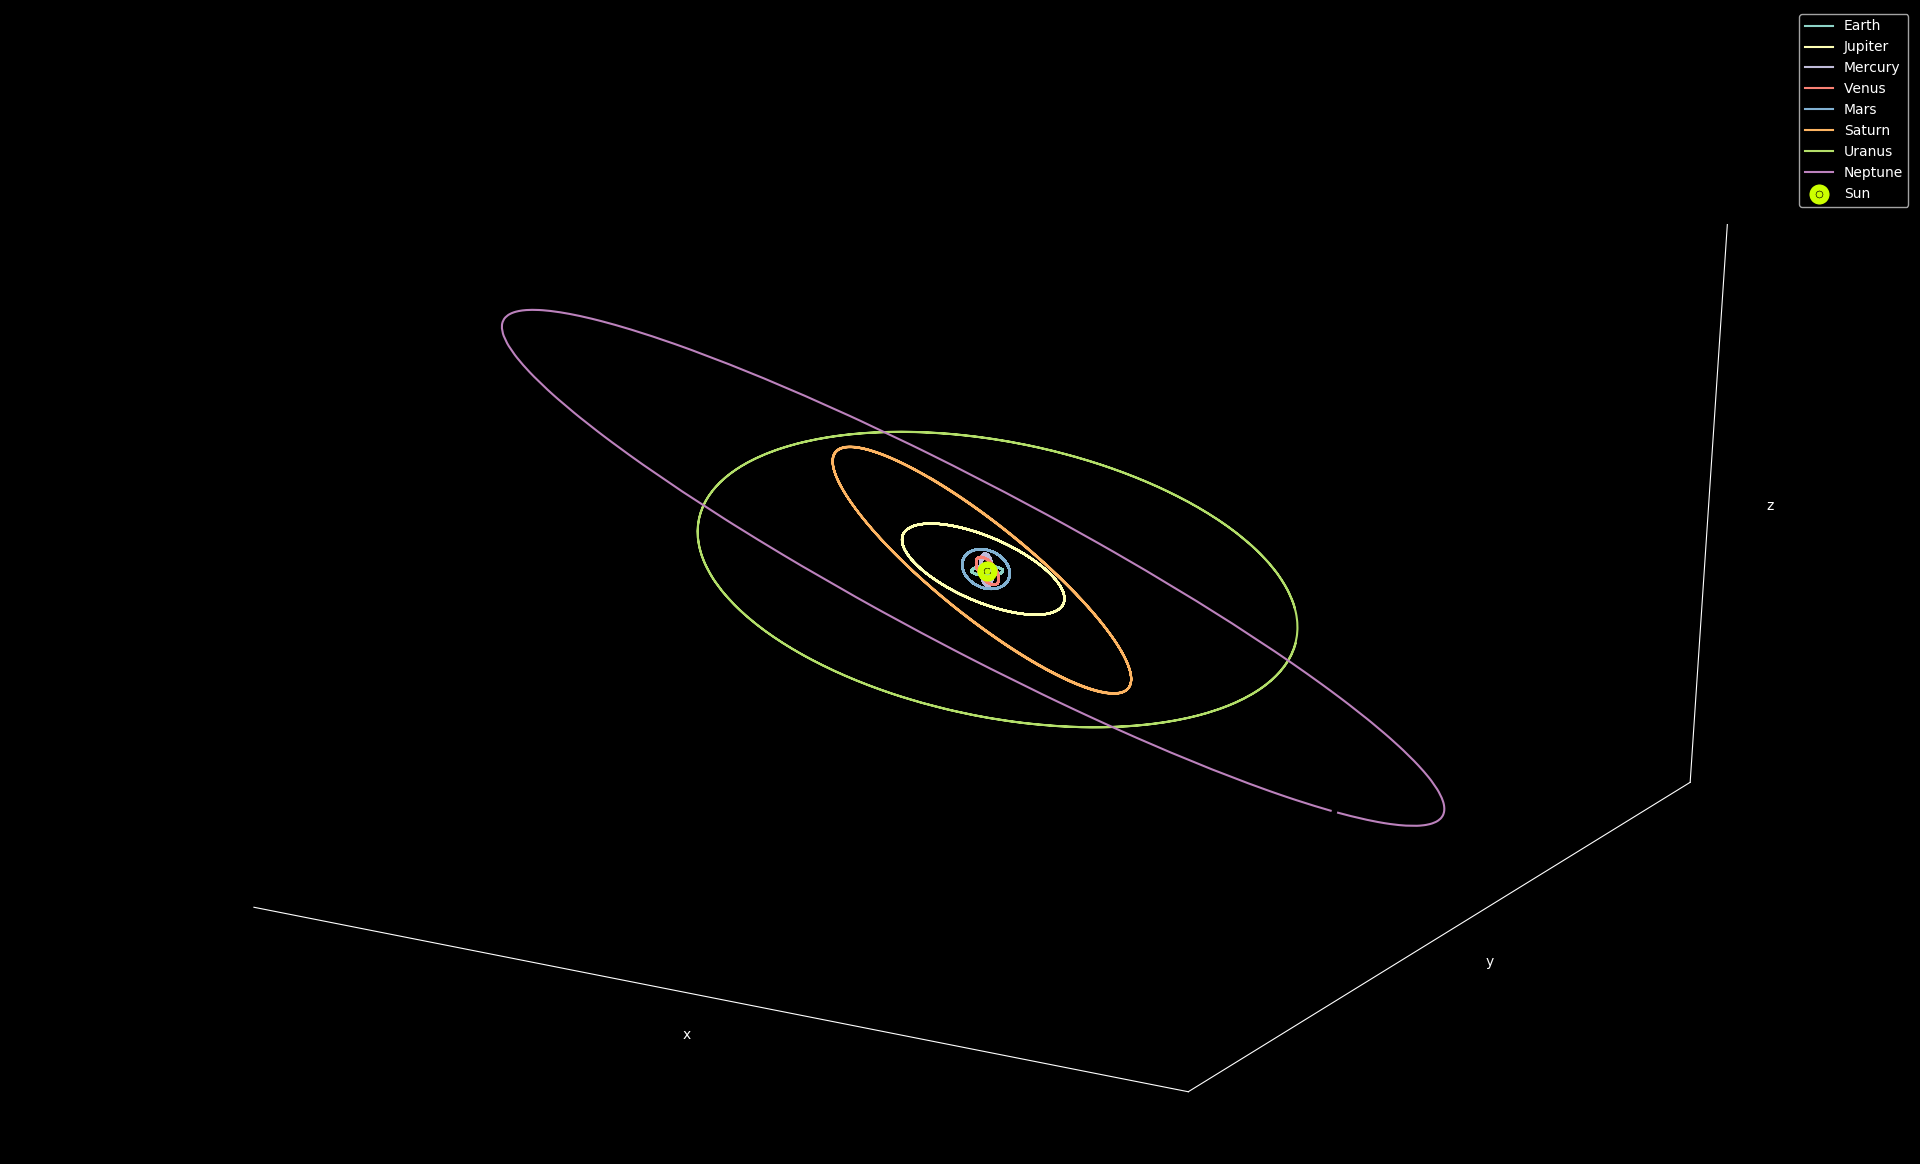
\includegraphics[width=0.8\textwidth]{./Plot/Solar_System.png}
        \caption{: Plot of the solar system.}
        \label{fig:solar}
    \end{center}
\end{figure}

From our results when testing the program, we see that if we don't fix the position of the sun, and give it the initial velocity it has according to the NASA initial values, the Sun moves toward the center of origin. In Figure \ref{fig:solar} we have fixed the Sun, as explained in the Programming section, with very similar results, with no visible differences in the plots.


\subsection{Perihelion of Mercury}
perihelion:
The speed of Mercury at perihelion is 12.44 AU/yr, and the distance to the sun at perihelion is 0.3075 AU.

sjekke at endringen i perihelion med en ren newton kraft (uten relativistiks) er minst et par ganger mindre enn den observerte Perihelion precession of mercury

\section{Discussion}
We have seen that the velocity Verlet method is more efficient for solving the coupled differential equations.
%Forskjeller mellom Verlet og Euler når vi tester algoritmene
%Time de og

%Can the obserevd perihelion precession of Mercury be explained by the general theory of relativity?

\section{Conclusion}


\section{Bibliography}


\begin{figure}[H]
    \begin{center}
        \includegraphics[width=0.8\textwidth]{./Plot/}
        \caption{: }
        \label{}
    \end{center}
\end{figure}

\href{https://en.wikipedia.org/wiki/Escape_velocity}{Escape velocity from Wikipedia}



\end{document}
